\documentclass{article}
%%%%%%%%%%%%%%%%%%%%%%%%%%%%% Define Article %%%%%%%%%%%%%%%%%%%%%%%%%%%%%%%%%%
%%%%%%%%%%%%%%%%%%%%%%%%%%%%%%%%%%%%%%%%%%%%%%%%%%%%%%%%%%%%%%%%%%%%%%%%%%%%%%%

%%%%%%%%%%%%%%%%%%%%%%%%%%%%% Using Packages %%%%%%%%%%%%%%%%%%%%%%%%%%%%%%%%%%
\usepackage{float}
\usepackage[letterpaper,portrait]{geometry}
\usepackage{graphicx}
\usepackage{anysize}
\usepackage{lipsum}
\usepackage{amsmath,amssymb,amsthm}
\usepackage[utf8]{inputenc}
\usepackage{multirow}
\usepackage{csquotes}
\usepackage[spanish]{babel}
\usepackage{apacite}
\usepackage{multicol}
\usepackage{parskip}
\usepackage{setspace}
\usepackage{empheq}
\usepackage{mdframed}
\usepackage{booktabs}
\usepackage{lipsum}
\usepackage{graphicx}
\usepackage{color}
\usepackage{psfrag}
\usepackage{pgfplots}
\usepackage{bm}
\usepackage{tocloft}
\usepackage{lscape}
\usepackage{adjustbox}
%%%%%%%%%%%%%%%%%%%%%%%%%%%%%%%%%%%%%%%%%%%%%%%%%%%%%%%%%%%%%%%%%%%%%%%%%%%%%%%

% Other Settings

%%%%%%%%%%%%%%%%%%%%%%%%%% Page Setting %%%%%%%%%%%%%%%%%%%%%%%%%%%%%%%%%%%%%%%
\geometry{letterpaper, margin=2.54cm}

%%%%%%%%%%%%%%%%%%%%%%%%%% Define some useful colors %%%%%%%%%%%%%%%%%%%%%%%%%%
\definecolor{ocre}{RGB}{243,102,25}
\definecolor{mygray}{RGB}{243,243,244}
\definecolor{deepGreen}{RGB}{26,111,0}
\definecolor{shallowGreen}{RGB}{235,255,255}
\definecolor{deepBlue}{RGB}{61,124,222}
\definecolor{shallowBlue}{RGB}{235,249,255}
%%%%%%%%%%%%%%%%%%%%%%%%%%%%%%%%%%%%%%%%%%%%%%%%%%%%%%%%%%%%%%%%%%%%%%%%%%%%%%%

%%%%%%%%%%%%%%%%%%%%%%%%%% Define an orangebox command %%%%%%%%%%%%%%%%%%%%%%%%
\newcommand\orangebox[1]{\fcolorbox{ocre}{mygray}{\hspace{1em}#1\hspace{1em}}}
%%%%%%%%%%%%%%%%%%%%%%%%%%%%%%%%%%%%%%%%%%%%%%%%%%%%%%%%%%%%%%%%%%%%%%%%%%%%%%%

%%%%%%%%%%%%%%%%%%%%%%%%%%%% English Environments %%%%%%%%%%%%%%%%%%%%%%%%%%%%%
\newtheoremstyle{mytheoremstyle}{3pt}{3pt}{\normalfont}{0cm}{\rmfamily\bfseries}{}{1em}{{\color{black}\thmname{#1}~\thmnumber{#2}}\thmnote{\,--\,#3}}
\newtheoremstyle{myproblemstyle}{3pt}{3pt}{\normalfont}{0cm}{\rmfamily\bfseries}{}{1em}{{\color{black}\thmname{#1}~\thmnumber{#2}}\thmnote{\,--\,#3}}
\theoremstyle{mytheoremstyle}
\newmdtheoremenv[linewidth=1pt,backgroundcolor=shallowGreen,linecolor=deepGreen,leftmargin=0pt,innerleftmargin=20pt,innerrightmargin=20pt,]{theorem}{Theorem}[section]
\theoremstyle{mytheoremstyle}
\newmdtheoremenv[linewidth=1pt,backgroundcolor=shallowBlue,linecolor=deepBlue,leftmargin=0pt,innerleftmargin=20pt,innerrightmargin=20pt,]{definition}{Definition}[section]
\theoremstyle{myproblemstyle}
\newmdtheoremenv[linecolor=black,leftmargin=0pt,innerleftmargin=10pt,innerrightmargin=10pt,]{problem}{Problem}[section]
%%%%%%%%%%%%%%%%%%%%%%%%%%%%%%%%%%%%%%%%%%%%%%%%%%%%%%%%%%%%%%%%%%%%%%%%%%%%%%%

%%%%%%%%%%%%%%%%%%%%%%%%%%%%%%% Plotting Settings %%%%%%%%%%%%%%%%%%%%%%%%%%%%%
\usepgfplotslibrary{colorbrewer}
\pgfplotsset{width=8cm,compat=1.9}
%%%%%%%%%%%%%%%%%%%%%%%%%%%%%%%%%%%%%%%%%%%%%%%%%%%%%%%%%%%%%%%%%%%%%%%%%%%%%%%

%%%%%%%%%%%%%%%%%%%%%%%%%%%%%%% Title & Author %%%%%%%%%%%%%%%%%%%%%%%%%%%%%%%%
\author{Gustavo Vergara}
%%%%%%%%%%%%%%%%%%%%%%%%%%%%%%%%%%%%%%%%%%%%%%%%%%%%%%%%%%%%%%%%%%%%%%%%%%%%%%%

\begin{document}
\pgfplotsset{compat=1.18}
\setstretch{2}

\begin{titlepage}
	\centering
	\vspace{2.5cm}
	{\scshape \Large TALLER INSTRUMENTOS \par}
	\vspace{5cm}
	\textbf\large\scshape{\par}
	\vspace{0.5cm}

	{\Large Vergara Pareja Gustavo\par}
	\vspace{5cm}
	{\scshape\Large Miguel Ángel Lancheros\par}
	\vspace{0.3cm}
	{\scshape\Large Metrología y Control de Calidad - G1IM \par}
	\vspace{0.3cm}
	{\scshape\Large Universidad de Córdoba\par}
	\vspace{0.3cm}
	{\Large \today \par}
\end{titlepage}
%\tableofcontents
\newpage

\section{¿Qué es el calibrador Vernier o pie de rey?}
Es un instrumento de medida de uso muy común por su fácil manejo y el grado de precisión en las mediciones realizadas. Básicamente, consta de una regla (graduada en milímetros) con una escuadra o tacón en el origen que determina la boca fija, sobre la que se desplaza
una pequeña regla móvil (nonio) que en su origen determina la boca móvil. El calibrador típico puede tomar tres tipos de mediciones: exteriores,
interiores y profundidades, pero algunos además pueden realizar medición de peldaño.
\begin{enumerate}
	\item ¿Cuántos modelos de vernier existen?\newline
	      Los vernier se clasifican en tres tipos, el estándar, largo y en pulgadas.
	      \begin{itemize}
		      \item Vernier estándar \newline
		            Este tipo de vernier es el más comúnmente utilizado, tiene n divisiones iguales
		            que ocupan la misma longitud que n-1 divisiones sobre la escala principal.
		            \begin{figure}[H]
			            \centering
			            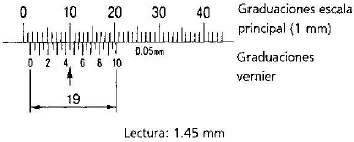
\includegraphics[width=0.6\textwidth]{lectura_vernier.png}
			            \caption{Vernier estándar}
			            \label{fig:imagen2}
		            \end{figure}
	      \end{itemize}

	      \begin{itemize}
		      \item Vernier largo \newline
		            El vernier largo está diseñado para que las graduaciones adyacentes sean más
		            fáciles de distinguir.
		            \begin{figure}[H]
			            \centering
			            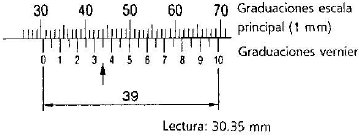
\includegraphics[width=0.6\textwidth]{lectura2.png}
			            \caption{Vernier Largo}
			            \label{fig:imagen2}
		            \end{figure}
	      \end{itemize}

	      \begin{itemize}
		      \item Vernier en pulgadas
		            \newline
		            El vernier en pulgadas utiliza la misma metododología del vernier estandar.
		            \begin{figure}[H]
			            \centering
			            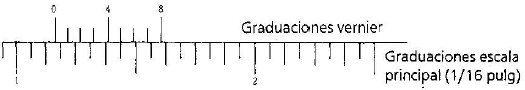
\includegraphics[width=0.6\textwidth]{vpulg.png}
			            \caption{Vernier en pulgadas}
			            \label{fig:imagen2}
		            \end{figure}
	      \end{itemize}

	\item ¿Para qué sirve cada uno?\newline
	      Si nos referimos a modelos, hay dos: analógico y electrodigital
	      \begin{itemize}
		      \item Vernier analogico \newline
		            Este tipo de calibrador tiene una escala vernier que debe leerse manualmente.
		            \begin{figure}[H]
			            \centering
			            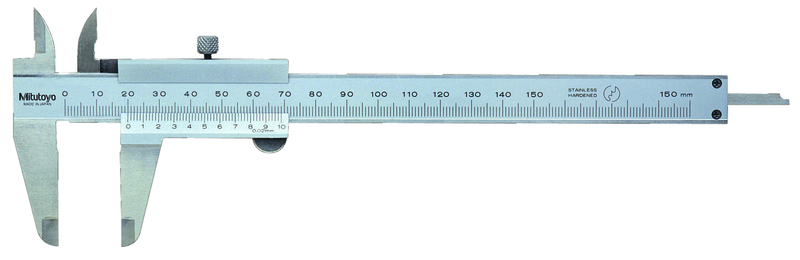
\includegraphics[width=0.6\textwidth]{ss.png}
			            \caption{Vernier analógico}
			            \label{fig:imagen2}
		            \end{figure}
	      \end{itemize}
	      \begin{itemize}

		      \item Vernier electrodigital \newline
		            Este tipo de calibrador tiene una pantalla electrodigital que muestra la medida directamente.
		            \begin{figure}[H]
			            \centering
			            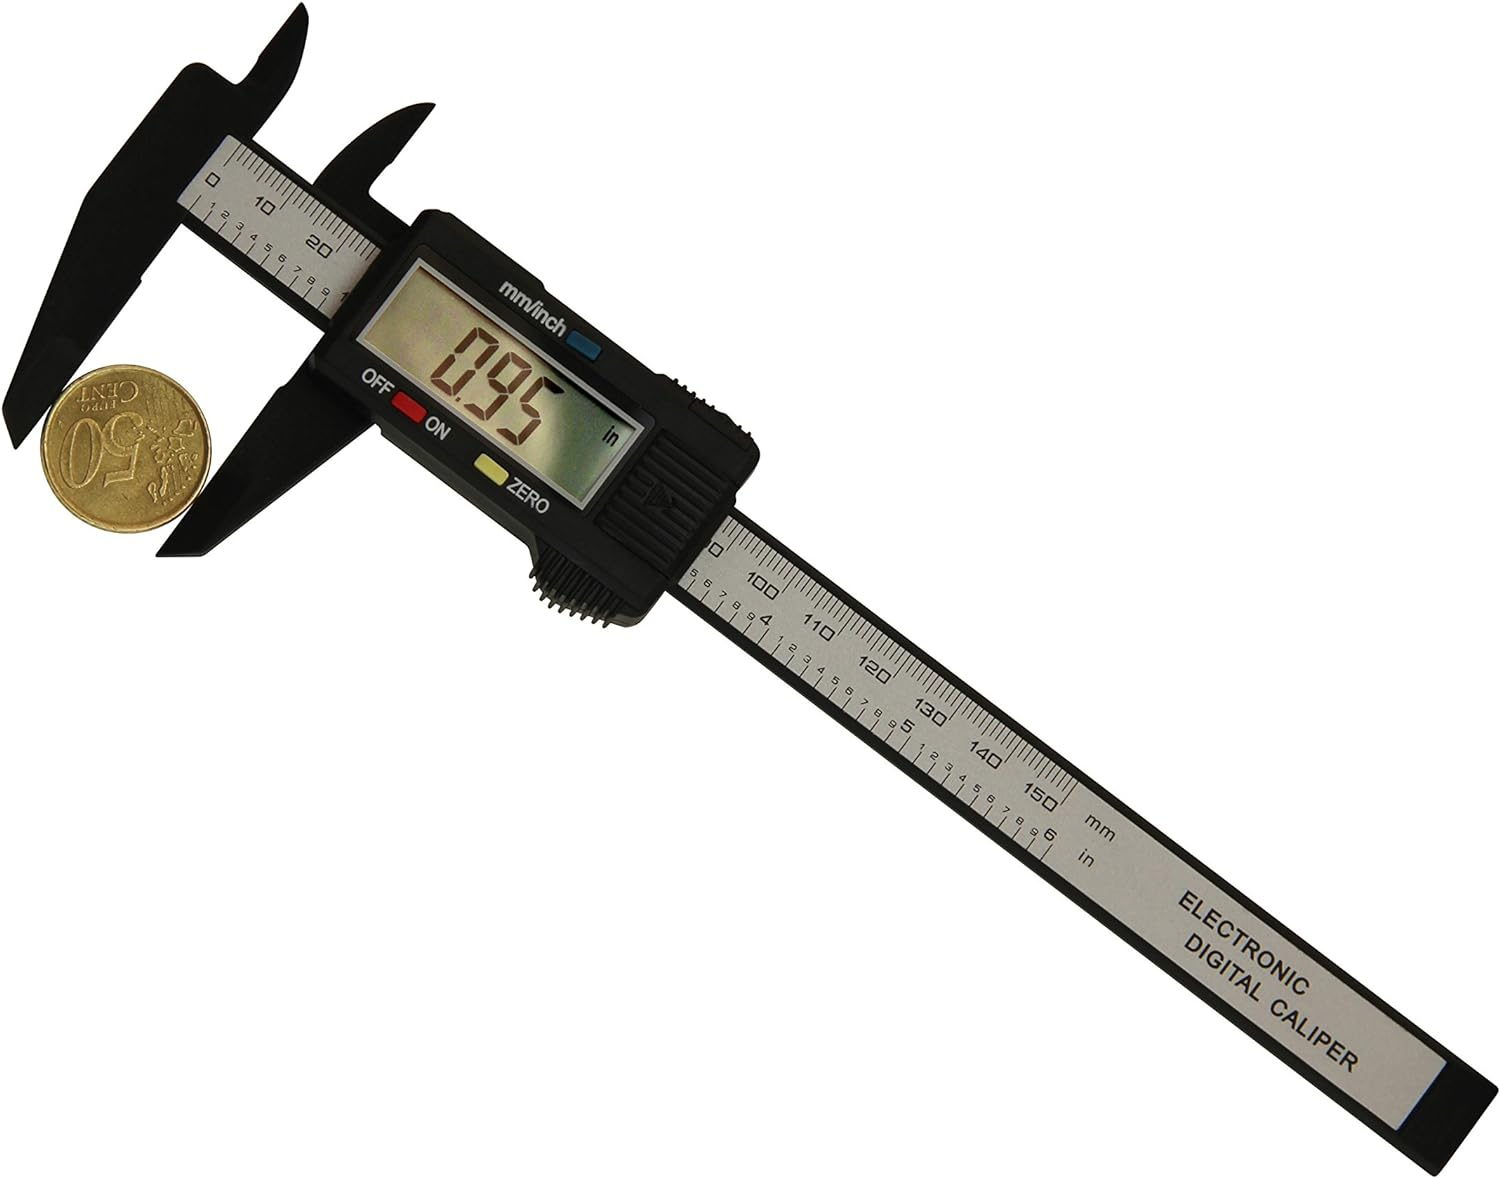
\includegraphics[width=0.4\textwidth]{digi.jpg}
			            \caption{Vernier electrodigital}
			            \label{fig:imagen2}
		            \end{figure}
	      \end{itemize}
	      \newpage

	\item ¿Cuáles son sus partes?

	      \begin{figure}[H]
		      \centering
		      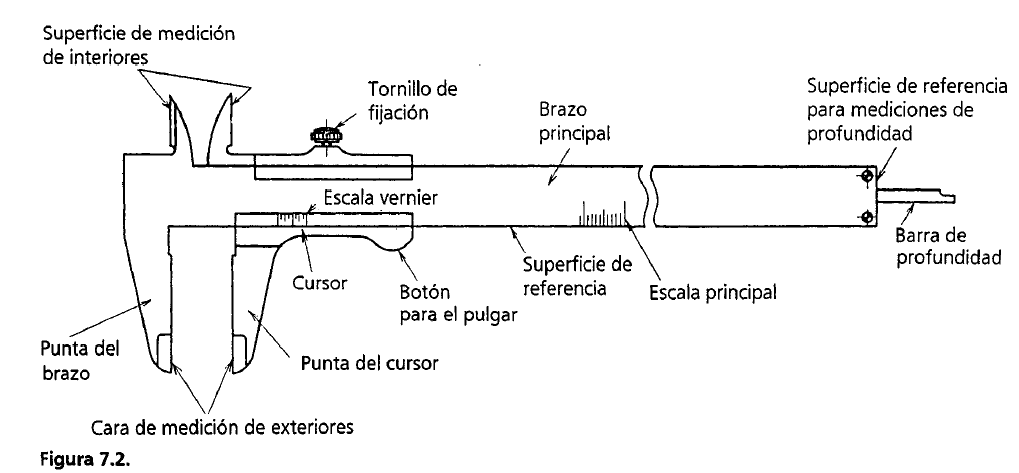
\includegraphics[width=1\textwidth]{partes_vernier.png}
		      \caption{Partes vernier analógico}
		      \label{fig:imagen2}
	      \end{figure}
	      \begin{figure}[H]
		      \centering
		      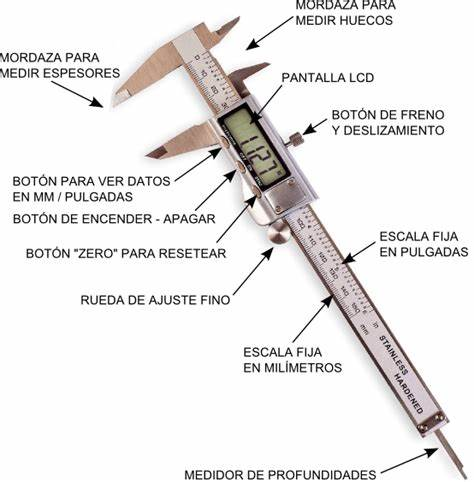
\includegraphics[width=0.7\textwidth]{partes_vernier.jpeg}
		      \caption{Partes vernier electrodigital}
		      \label{fig:imagen2}
	      \end{figure}
	\item ¿Cómo se lee la medida en el instrumento?\newline
	      Para leer la medida en el calibrador Vernier, se deben seguir estos pasos dependiento del tipo de medición:
	      \begin{itemize}
		      \item Para exteriores:
		            \begin{itemize}
			            \item Mantenga y mida la pieza de trabajo en una posición
			                  tan cercana a la superficie de referencia como sea
			                  posible.
			            \item Asegúrese de que las caras de medición exterior hagan
			                  contacto adecuado con la pieza por medir.
			                  \begin{figure}[H]
				                  \centering
				                  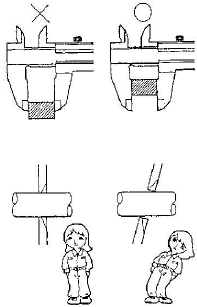
\includegraphics[width=0.2\textwidth]{ext.png}
				                  \caption{Medida exteriores}
				                  \label{fig:imagen2}
			                  \end{figure}
		            \end{itemize}
		      \item Para interiores: \newline
		            Tome la medida cuando las puntas de medición de interiores
		            estén tan adentro de la pieza como sea posible.
		            \begin{itemize}
			            \item Cuando mida un diámetro interior lea la escala mientras
			                  el valor indicado esté en su máximo.
			            \item Cuando mida el ancho de una ranura, lea la escala
			                  mientras el valor indicado esté en su mínimo.
			                  \begin{figure}[H]
				                  \centering
				                  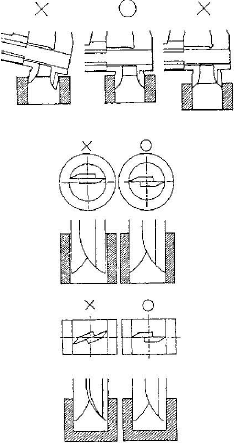
\includegraphics[width=0.28\textwidth]{int.png}
				                  \caption{Medida interiores}
				                  \label{fig:imagen2}
			                  \end{figure}
		            \end{itemize}
		      \item Para profundidad:
		            \begin{itemize}
			            \item Tome la medida cuando la cara inferior del cuerpo
			                  principal esté en contacto uniforme con la pieza de
			                  trabajo.
			                  \begin{figure}[H]
				                  \centering
				                  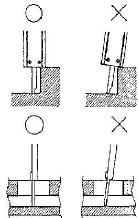
\includegraphics[width=0.28\textwidth]{prof.png}
				                  \caption{Medida profundidad}
				                  \label{fig:imagen2}
			                  \end{figure}
		            \end{itemize}
	      \end{itemize}

\end{enumerate}\newpage
Para leer la medida en el calibrador Vernier, se deben seguir estos pasos:

\begin{enumerate}
	\item Ajustar el brazo móvil para que la colisa o la punta de profundidad entre en contacto con la pieza que se va a medir.
	\item Leer la medida en la escala principal.
	\item Buscar la marca vernier que coincide con el cero de la escala principal.
	\item La lectura vernier es la diferencia entre la marca vernier y la marca principal más cercana.
\end{enumerate}


\section{¿Qué es el micrómetro?}
El micrómetro es un instrumento
de medida directa de precisión, que consigue una
gran exactitud en las mediciones efectuadas. En líneas
generales el micrómetro consta de un cilindro "fijo"
graduado en milímetros, sobre el que se desplaza un
cilindro exterior o tambor (a través de un mecanismo
tipo "husillo"), cuya división en partes determina la precisión
del instrumento.
\begin{itemize}
	\item¿Cuántos modelos de micrómetros existen?
	      \begin{itemize}
		      \item Micrómetros para tubo
		      \item Micrómetro para ranuras
		      \item Micrómetro de puntas
		      \item Micrómetros para ceja de latas
		      \item Micrómetro de exteriores con husillo no giratorio
		      \item Micrómetro con topes del arco en V
		      \item Micrómetros para espesor de láminas
		      \item Micrómetro para dientes de engrane
	      \end{itemize}
	      \newpage
	\item¿Para qué sirve cada uno?
	      \begin{itemize}
		      \item Micrómetros para tubo\newline
		            Los micrómetros para tubo se utilizan para medir el diámetro exterior de tubos. Tienen una punta especial que se ajusta a la forma del tubo para proporcionar una medición precisa.

		      \item Micrómetro para ranuras\newline
		            Los micrómetros para ranuras se utilizan para medir el ancho o la profundidad de una ranura. Tienen una punta especial que se desliza en la ranura para proporcionar una medición precisa.
		      \item Micrómetro de puntas\newline
		            Los micrómetros de puntas se utilizan para medir el diámetro interior o exterior de una pieza. Tienen dos puntas que se presionan contra la pieza para proporcionar una medición precisa.
		      \item Micrómetros para ceja de latas \newline
		            Los micrómetros para ceja de latas se utilizan para medir el ancho o la altura de la ceja de una lata. Tienen una punta especial que se ajusta a la forma de la ceja para proporcionar una medición precisa.

		      \item Micrómetro de exteriores con husillo no giratorio\newline
		            Los micrómetros de exteriores con husillo no giratorio tienen un husillo que no gira. Esto permite realizar mediciones de precisión en piezas que son difíciles de sujetar.
		      \item Micrómetro con topes del arco en V\newline
		            Los micrómetros con topes del arco en V tienen topes en forma de arco en V. Esto permite realizar mediciones de precisión en piezas que tienen superficies curvas.
		      \item Micrómetros para espesor de láminas\newline
		            Los micrómetros para espesor de láminas se utilizan para medir el espesor de una lámina. Tienen una punta especial que se desliza entre las capas de la lámina para proporcionar una medición precisa.
		      \item Micrómetro para dientes de engrane\newline
		            Los micrómetros para dientes de engrane se utilizan para medir el paso de los dientes de un engranaje. Tienen una punta especial que se desliza entre los dientes para proporcionar una medición precisa.

	      \end{itemize}


	\item ¿Cuáles son sus partes?
	      \begin{figure}[H]
		      \centering
		      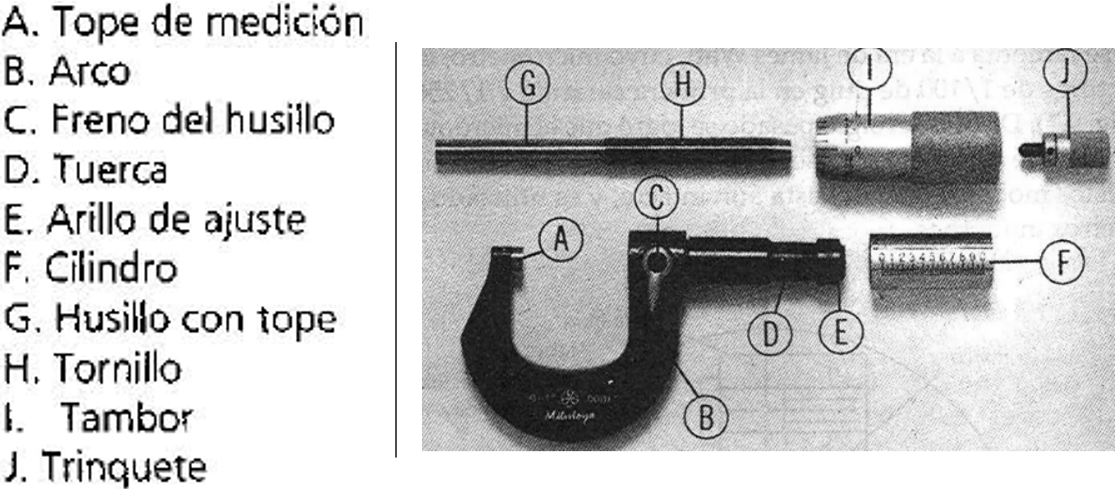
\includegraphics[width=0.7\textwidth]{micrometro.png}
		      \caption{Partes micrometro}
		      \label{fig:imagen2}
	      \end{figure}

	\item¿Cómo se lee la medida en el instrumento?

	      Para leer la medida en el micrómetro, se deben seguir estos pasos:
	      \begin{enumerate}
		      \item Ajustar el tornillo micrométrico para que las cuñas entren en contacto con la pieza que se va a medir.
		      \item Leer la medida en el tambor graduado.
		      \item La lectura es la suma de la lectura en la escala principal y la lectura en el tambor graduado.
	      \end{enumerate}





\newpage
\end{itemize}
\bibliographystyle{apacite}
\nocite{*}
\bibliography{instrumentos}

\end{document}